\documentclass[journal,12pt,onecolumn]{IEEEtran}
\usepackage{cite}
\usepackage{caption}
\usepackage{graphicx}
\usepackage{amsmath,amssymb,amsfonts,amsthm}
\usepackage{algorithmic}
\usepackage{graphicx}
\usepackage{textcomp}
\usepackage{xcolor}
\usepackage{tfrupee}
\usepackage{txfonts}
\usepackage{listings}
\usepackage{enumitem}
\usepackage{mathtools}
\usepackage{gensymb}
\usepackage{comment}
\usepackage[breaklinks=true]{hyperref}
\usepackage{tkz-euclide} 
\usepackage{listings}
\usepackage{gvv}
%\def\inputGnumericTable{}
\usepackage[latin1]{inputenc} 
\usetikzlibrary{arrows.meta, positioning}
\usepackage{xparse}
\usepackage{color}                                            
\usepackage{array}                                            
\usepackage{longtable}                                       
\usepackage{calc}                                             
\usepackage{multirow}
\usepackage{multicol}
\usepackage{hhline}                                           
\usepackage{ifthen}                                           
\usepackage{lscape}
\usepackage{tabularx}
\usepackage{array}
\usepackage{float}
\usepackage{marvosym}
\usepackage{float}
%\newcommand{\define}{\stackrel{\triangle}{=}}
\theoremstyle{remark}
\usepackage{circuitikz}
\captionsetup{justification=centering}
\usepackage{tikz}

\title{Matrices in Geometry 10.7.86}
\author{EE25BTECH11037 - Divyansh}
\begin{document}
\vspace{3cm}
\maketitle
{\let\newpage\relax\maketitle}
\textbf{Question: }
Let $\vec{C_1}$ and $\vec{C_2}$ be two circles with $\vec{C_2}$ lying inside $\vec{C_1}$. A circle $C$ lying inside $\vec{C_1}$ touches $\vec{C_1}$ internally and $\vec{C_2}$ externally. Identify the locus of center of $\vec{C}$.
\vspace{2mm}


\textbf{Solution:}
Let the center of $\vec{C}$, $\vec{C_1}$ and $\vec{C_2}$ be $\vec{O}$, $\vec{O_1}$ and $\vec{O_2}$, respectively.\\
Let the radii of circles $\vec{C}$, $\vec{C_1}$ and $\vec{C_2}$ be $r$, $r_1$ and $r_2$ \\
It is given that $\vec{C}$ touches the circle $\vec{C_1}$ internally and $\vec{C_2}$ externally. Therefore, 
\begin{align}
    \norm{\vec{O} - \vec{O_1}} = r_1 - r\\
    \norm{\vec{O} - \vec{O_2}} = r_2 + r
\end{align}
Adding these two equations, we get 
\begin{align}
    \norm{\vec{O} - \vec{O_1}} + \norm{\vec{O} - \vec{O_2}} = r_1 + r_2
\end{align}
Substitute $\vec{O}$ as $\vec{x}$
\begin{align}
    \norm{\vec{x} - \vec{O_1}} + \norm{\vec{x} - \vec{O_2}} = r_1 + r_2
\end{align}
This is the equation of an ellipse because it is of form 
\begin{align}
    \norm{\vec{x} - \vec{S_1}} + \norm{\vec{x} - \vec{S_2}} = 2a
\end{align}
with foci  as $\vec{O_1}$ , $\vec{O_2}$ and length of the major axis as $r_1 + r_2$.
\begin{align}
    \norm{\vec{x} - \vec{O_1}} + \norm{\vec{x} - \vec{O_2}} = K, \ K=r_1+r_2
\end{align}
To eliminate square roots from the norms, we rearrange and square the equation.
\begin{align}
 \norm{\vec{x} - \vec{O_1}} = K - \norm{\vec{x} - \vec{O_2}}
\end{align}
Squaring both sides and using the property $\norm{\vec{v}}^2 = \vec{v}^{\top}\vec{v}$:
\begin{align}
 \norm{\vec{x} - \vec{O_1}}^2 = \brak{K - \norm{\vec{x} - \vec{O_2}}}^2
\end{align}
\begin{align}
 \brak{\vec{x} - \vec{O_1}}^{\top}\brak{\vec{x} - \vec{O_1}} = K^2 - 2K\norm{\vec{x} - \vec{O_2}} + \norm{\vec{x} - \vec{O_2}}^2
\end{align}
Expanding the terms and simplifying gives the following.
\begin{align}
 \norm{\vec{x}}^2 - 2\vec{O_1}^{\top}\vec{x} + \norm{\vec{O_1}}^2 = K^2 - 2K\norm{\vec{x} - \vec{O_2}} + \norm{\vec{x}}^2 - 2\vec{O_2}^{\top}\vec{x} + \norm{\vec{O_2}}^2
\end{align}
Rearrange the equation to isolate the remaining norm term:
\begin{align}
 2K\norm{\vec{x} - \vec{O_2}} = (K^2 + \norm{\vec{O_2}}^2 - \norm{\vec{O_1}}^2) + 2\brak{\vec{O_1} - \vec{O_2}}^{\top}\vec{x}
\end{align}
Let $S = K^2 + \norm{\vec{O_2}}^2 - \norm{\vec{O_1}}^2$ and $\vec{v} = 2\brak{\vec{O_1} - \vec{O_2}}$. The equation becomes:
\begin{align}
 2K\norm{\vec{x} - \vec{O_2}} = S + \vec{v}^{\top}\vec{x}
\end{align}
Squaring both sides again:
\begin{align}
 4K^2\norm{\vec{x} - \vec{O_2}}^2 = (S + \vec{v}^{\top}\vec{x})^2
\end{align}
\begin{align}
 4K^2\brak{\vec{x}^{\top}\vec{x} - 2\vec{O_2}^{\top}\vec{x} + \norm{\vec{O_2}}^2} = S^2 + 2S\brak{\vec{v}^{\top}\vec{x}} + \brak{\vec{v}^{\top}\vec{x}}^2
\end{align}
Using the identity $\brak{\vec{v}^{\top}\vec{x}}^2 = \vec{x}^{\top}\brak{\vec{v}\vec{v}^{\top}}\vec{x}$, we group all terms to one side to match the form $\vec{x}^{\top}V\vec{x} + 2\vec{u}^{\top}\vec{x} + f = 0$.
\begin{align}
 \vec{x}^{\top}\brak{4K^2I - \vec{v}\vec{v}^{\top}}\vec{x} + 2\brak{-4K^2\vec{O_2} - S\vec{v}}^{\top}\vec{x} + \brak{4K^2\norm{\vec{O_2}}^2 - S^2}= 0
\end{align}
Compared with the general conic equation, we identify the matrix $V$, the vector $\vec{u}$, and the scalar $f$:
\begin{align}
    \vec{V} &= 4K^2I - \vec{v}\vec{v}^{\top} = 4\brak{r_1 + r_2}^2I - 4\brak{\vec{O_1}-\vec{O_2}}\brak{\vec{O_1}-\vec{O_2}}^{\top} \\
    \vec{u} &= -4K^2\vec{O_2} - S\vec{v} = -4\brak{r_1 + r_2}^2\vec{O_2} - \brak{\brak{r_1 + r_2}^2 + \norm{\vec{O_2}}^2 - \norm{\vec{O_1}}^2 }\cdot 2\brak{\vec{O_1}-\vec{O_2}} \\
    f &= 4K^2\norm{\vec{O_2}}^2 - S^2 = 4\brak{r_1 + r_2}^2\norm{\vec{O_2}}^2 - \brak{\brak{r_1 + r_2}^2 + \norm{\vec{O_2}}^2 - \norm{\vec{O_1}}^2}^2
\end{align}
\begin{figure}[H]
    \centering
    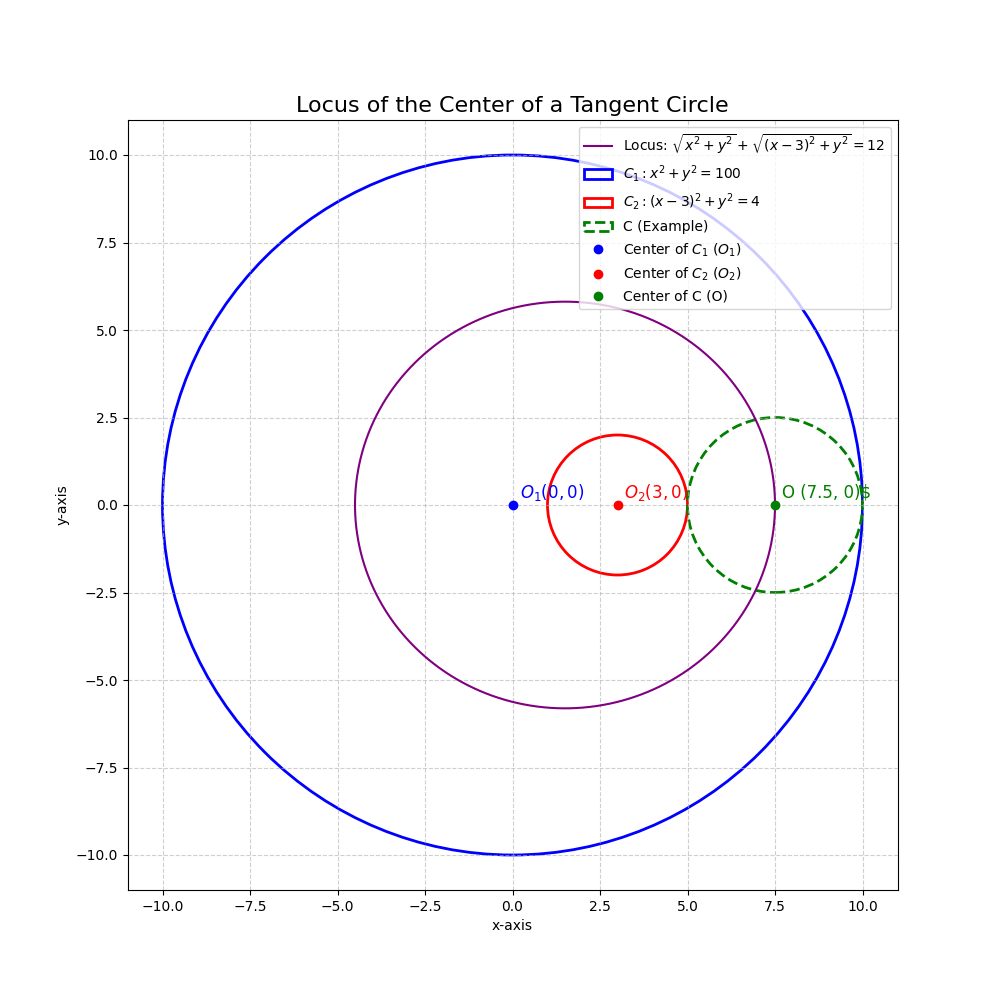
\includegraphics[width=0.7\columnwidth]{figs/1.png}
    \caption{Caption}
    \label{fig:placeholder}
\end{figure}
\end{document}

